\documentclass[dvisvgm,tikz,border=4pt]{standalone}
\usepackage{amsmath,amssymb}

\usetikzlibrary{arrows.meta,positioning,automata,shapes,shapes.misc,calc,decorations.pathmorphing,decorations.markings,angles,quotes,patterns,mindmap,matrix,knots,hobby,trees}
\tikzset{->-/.style={decoration={markings, mark=at position 0.5 with {\arrow{Stealth}}}, postaction={decorate}}}
\begin{document}
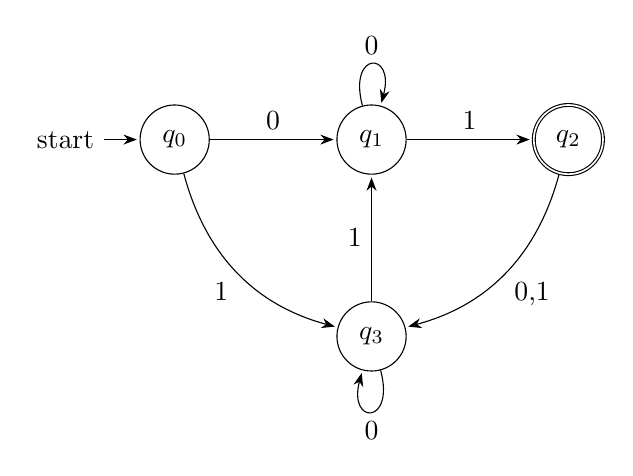
\begin{tikzpicture}[shorten >=1pt, node distance=2.5cm, on grid, auto, >=Stealth]
\node[state, initial] (q0) {$q_0$};
\node[state] (q1) [right=of q0] {$q_1$};
\node[state, accepting] (q2) [right=of q1] {$q_2$};
\node[state] (q3) [below=of q1] {$q_3$};
\path[->] (q0) edge node {0} (q1) edge [bend right] node[swap] {1} (q3)
          (q1) edge node {1} (q2) edge [loop above] node {0} ()
          (q2) edge [bend left] node {0,1} (q3)
          (q3) edge [loop below] node {0} () edge node {1} (q1);
\end{tikzpicture}
\end{document}
